\chapter{Approximation}\label{c-Approx}

Up till now we have dealt with interpolation, where we want to exactly match a set of points.  In reality, we are often more concerned with having a good overall approximation rather than an exact matching at a few points.  There are a lot of ways to approximate a function.  In general there are two main areas discrete and continuous.  We will cover the discrete case.  The continuous method involves some functional analysis and we do not have the time to cover it well.  If you are interested it can provide a fun project, and I have some good resources you can use.

\section{Least Squares Approximation}

We proceed with the discrete case.  The discrete case involves measuring the function to be approximated at a series of points, and then finding the best coefficients in some sense for some functions of interest.

Some sense?  What do I mean by that?  Well, put simply, there are a variety of different methods of measuring how good an approximation is.  The standard method is the one we will concentrate on, and it is called least squares.  As with many things in Math, least squares owes its basis to Gauss, who used it to calculate orbits of objects in the solar system \bb{cfg95}.  Numerous other works have covered solution methods \bb{bjorck88,lh95} and solved cases such as special structure \bb{cox81, cyb84}, sparse matrices \bb{duff74, gehe80}, and numerical issues \bb{bjorck96, cline73, pw70}.  Least squares assumes that the matrix, $A$ is known exactly ($E_{A} = 0$), and thus all errors occur in the observations, $b$, only.  It is sometimes also referred to as Errors-in-Observations, due to the assumption of the errors occurring only in $b$.  The basic idea is to reduce the sum of the squares of the distances from the measurements to the function to be fitted at each of the x values.  The problem can be stated as
\beq
\min_{x}\| Ax-b \|^{2}.
\eeq
The last point is very important because it is the basis of much of the problems in least squares.  In essence the answer you get is dependent on your choice of independent variables.  The key idea to get is that there are reasons to look beyond least squares.

Consider the problem of calibrating a gas thermometer.  Gas thermometers are based on Charles' law, which states that the volume of a fixed mass of gas at a fixed pressure is proportional to its temperature.  A simple gas thermometer can be made by trapping some gas with a mercury plug in a capillary tube that is open on only one end \bb{GenChem}.  The volume is thus proportional to the height of the plug.  The equation of the thermometer is thus $hc_{1}=T$, where $h$ is the height of the plug, $c_{1}$ is the constant we want to know, and $T$ is the absolute temperature.  We place the gas thermometer in a stirred liquid bath with a known thermometer.  We heat the bath and take height and temperature measurements at various times.  The LS solution gives us that $\hat c_{1}=h^{\dagger}T$, but we can see that this minimizes the error in the measured temperature, $T$, from the predicted temperature, $hh^{\dagger}T$.  By the same token we could use the relation $h=c_{2}T$, with $c_{2}=\frac{1}{c_{1}}$.  The LS solution, $\hat c_{2}=T^{\dagger}h$, thus minimizes the error between the measured height, $h$, and the predicted height $TT^{\dagger}h$.  A problem arises in the LS method in that generally $\hat c_{1}\ne\frac{1}{\hat c_{2}}$.  This can be seen easily in Figure~\ref{gastherm}.  The slope of the line designated temperature errors, is $\hat c_{1}$, while the slope of the line designated height errors is $\frac{1}{\hat c_{2}}$.  The line designated theoretical is the ``true'' system from which the estimates were generated.  It is easy to see that the slopes are not the same, and thus $\hat c_{1}\ne\frac{1}{\hat c_{2}}$.  The LS solution does not even perfectly handle the case where the system matrix is ``known'', which gives us cause to be concerned as to how it will perform when there are perturbations to the system matrix.

\begin{figure}[h]
\begin{center}
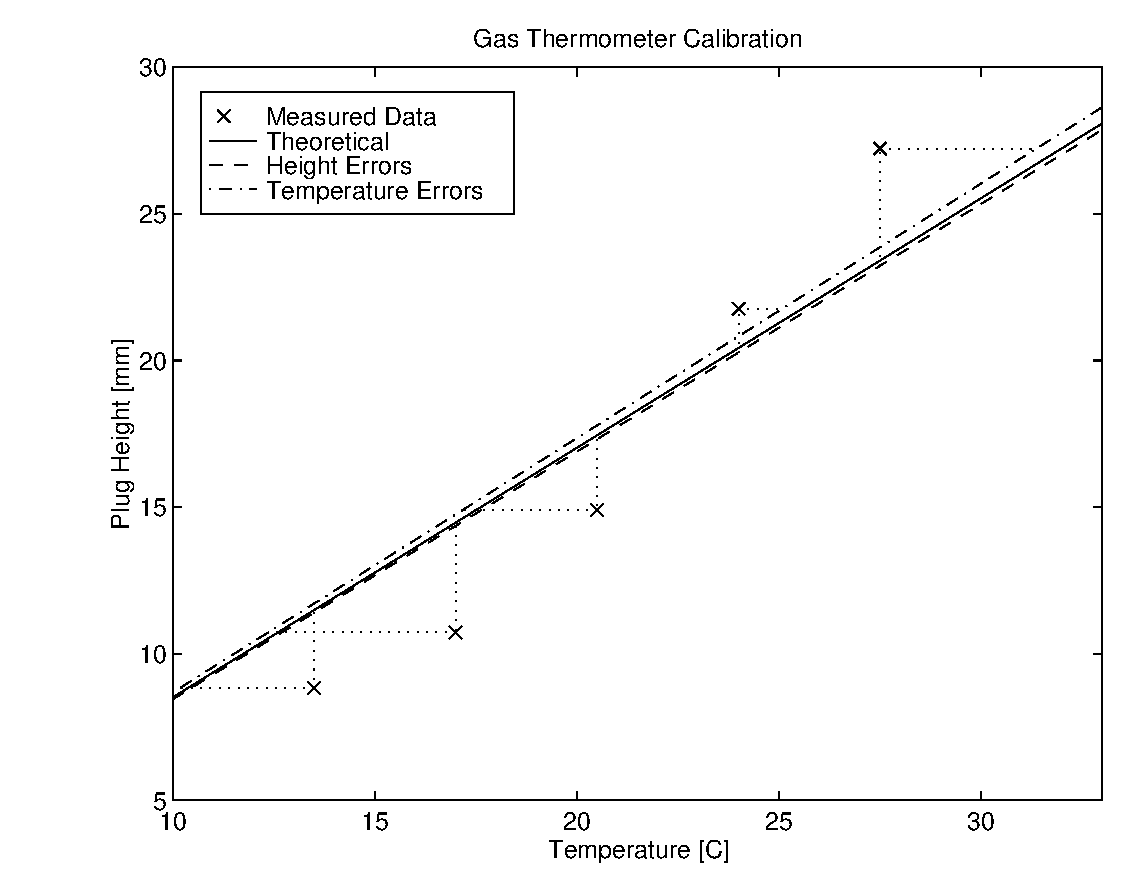
\includegraphics[width=4in]{gastherm.eps}
\end{center}
\caption{Gas Thermometer Example}
\label{gastherm}
\end{figure}

The most well known alternative to least squares is total least squares (TLS).  In TLS we look at the perpendicular distance to the function.  This handles many of the problems of least squares but is more sensitive to errors, as it is ``optimistic'' in how it looks at the problem.  A huge body of literature is dedicated to this problem, and this is the central area of my dissertation (available at www.r2labs.org).  While some of these other methods are very interesting, we will stick to least squares for the moment, but we will remember that problems can occur and so if we have problems we know there are things we can do.

Getting back to business we have a set of $m$ points $(x_{i},y_{i})$ and
a group of $n$ functions $\phi_{i}(x)$ that we want to use to
approximate the points with.  We thus have $m$ equations to find $n$
coefficients.
\beqn
y_{1} & - & \sum_{i=1}^{n}a_{i}\phi_{i}(x_{1}) \\
y_{2} & - & \sum_{i=1}^{n}a_{i}\phi_{i}(x_{2}) \\
& \vdots & \\
y_{m} & - & \sum_{i=1}^{n}a_{i}\phi_{i}(x_{m})
\eeqn
We can rewrite these into a matrix formulation, as
\beqn
Y-\Phi A \\
\eeqn
where
\beqn
Y & = & \left[\begin{matrix}y_{1} & y_{2} & \cdots & y_{m}\end{matrix}\right]^{T} \\
\Phi & = & \left[\begin{matrix}
\phi_{1}(x_{1}) & \phi_{2}(x_{1}) & \cdots & \phi_{n}(x_{1}) \cr
\phi_{1}(x_{2}) & \phi_{2}(x_{2}) & \cdots & \phi_{n}(x_{2}) \cr
\vdots          & \vdots          & \ddots & \vdots \cr
\phi_{1}(x_{m}) & \phi_{2}(x_{m}) & \cdots & \phi_{n}(x_{m})
\end{matrix}\right] \\
A & = & \left[\begin{matrix}a_{1} & a_{2} & \cdots & a_{m}\end{matrix}\right]^{T}.
\eeqn
At this point we want to minimize the square error which is what the
2-norm does, so we have $\min_{A}\| Y-\Phi A\|_{2}^{2}$ .  The norm we
are minimizing is called the
cost function.  The solution is given by $A=\Phi^{\dagger}Y$, where
$\Phi^{\dagger}$ is called the pseudo-inverse of $\Phi$.  Prove it?
Sure!  To avoid getting into some deeper areas of linear algebra we
will assume that $\Phi$ has linearly independent columns.  This is not
restrictive, as we usually have a lot of measurements and only a few
functions we want to fit to them ($m>>n$).

We recall from calculus that the minimum occurs when the gradient (derivative)
is zero. We thus take the gradient of the cost with respect to $A$ and
set it equal to zero to obtain
\beqn
0 & = &
\nabla_{A}\| Y-\Phi A\|_{2}^{2} \\
 & = &
\nabla_{A}(Y-\Phi A)^{T}(Y-\Phi A) \\
 & = &
-\Phi^{T}(Y-\Phi A) \\
 & = &
\Phi^{T}\Phi A-\Phi^{T}Y \\
\Phi^{T}Y
 & = &
\Phi^{T}\Phi A
\eeqn
The last line is what is referred to as the normal equation(s).  Note
that some pluralize it to reflect that the single matrix equation
reflects $n$ scalar equations.  I don't care, use what you like.  We
note that if $\Phi$ has linearly independent columns, then
$(\Phi^{T}\Phi)^{-1}$ exists.
\beqn
\Phi^{T}\Phi A
 & = &
\Phi^{T}Y \\
A
 & = &
(\Phi^{T}\Phi)^{-1}\Phi^{T}Y \\
A
 & = &
\Phi^{\dagger}Y
\eeqn
You might wonder how the last step works.  Some might just call it a definition but in reality it is because $(\Phi^{T}\Phi)^{-1}\Phi^{T}$ satisfies the four conditions of a pseudo inverse (called the Penrose conditions).
\begin{enumerate}
\item $\Phi\Phi^{\dagger}\Phi=\Phi$
\item $\Phi^{\dagger}\Phi\Phi^{\dagger}=\Phi^{\dagger}$
\item $\Phi\Phi^{\dagger}=(\Phi\Phi^{\dagger})^{T}$
\item $\Phi^{\dagger}\Phi=(\Phi^{\dagger}\Phi)^{T}$
\end{enumerate}
The properties are simple and easy to check, and yes, you have to check all four.  Many times a candidate matrix fails only one of them.  The first two properties tell us that it correctly maps the range spaces from the fundamental theorem of linear algebra, and the second two tell us the composite maps are symmetric.  The pseudo-inverse always exists and is unique.  Additionally, when the true inverse exists, it is the pseudo-inverse.  These are just a few of the many reasons to love the pseudo-inverse\ldots

The result is established.  The nice thing about how we have handled things here is we have not specified what the functions are (they have to be linearly independent but that is no problem) or how many of them we want to fit.  You can now fit any combination of functions you like.

The solution is the same for a deterministic assumption, as for an assumption that additive zero mean gaussian noise is present in the measurements, $b$.  The solution can be thought of as the projection of $b$ into the range of $A$, as seen in Figure~\ref{f-geo-ls}.  The cost criterion is appealing to physical intuition, since it requires the solution to account for all of the measurements the system could have produced.  The solution only requires the basic data (system matrix and measurements), and the complexity of the solution is the standard of comparison.  It is easy see why the least squares criterion is popular, but it is not without its problems.  The choice of independent variables, which will be shown below, and scaling problems, which are outlined in \bb{Mendel95}, are few of the well known problems with least squares.
\begin{figure}
\begin{center}
  {\tt    \setlength{\unitlength}{0.92pt}
\begin{picture}(260,185)
\thinlines    \put(69,35){$Ax_{ls}$}
              \put(105,104){$Ax_{ls}-b$}
              \put(164,55){$Ax$}
              \put(86,166){$b$}
              \put(86,163){\line(1,-4){31}}
              \put(12,12){\vector(1,2){75}}
              \put(12,12){\vector(4,1){151}}
              \put(12,12){\vector(0,1){157}}
              \put(13,12){\vector(1,0){237}}
\end{picture}}
\end{center}
\caption{Geometric Interpretation of Least Squares Solution}
\label{f-geo-ls}
\end{figure}

As an example let's look at linear least squares for the points (0,1), (1,2), and (2,3).  We need to find the coefficients $m$, and $b$ for the line.  We construct our matrices
\beqn
Y & = & \left[\begin{matrix}1 & 2 & 3\end{matrix}\right]^{T} \\
\Phi & = & \left[\begin{matrix}
1 & 1 & 1 \cr
0 & 1 & 2
\end{matrix}\right]^{T} \\
A & = & \left[\begin{matrix}b & m\end{matrix}\right]^{T}.
\eeqn

As a second example, consider fitting $e^{ax}$ to (0,1), (1,.5), and
(2,.25).  To separate the coefficient, $a$, from the variable, $x$ we
take the natural log of $y_{i}=e^{ax_{i}}$ to obtain $\ln(y_{i})=ax$.
We can proceed as before now.

As a third example we will consider the second problem where we have
noise (random errors) in the measurements.  These three examples are
coded into Matlab by
\SciLab{Matlab code for examples}{code:LS_example}{scilab/LS_example.m}
and we get the output below and in Fig~\ref{llsqex}.
\begin{list}{}{\leftmargin=3em}\item[]
\begin{verbatim}
A =
    1.0000
    1.0000
ans =
    0
Ae =
   -0.6931
Aee =
   -0.4650
\end{verbatim}
\end{list}

\begin{figure}[h]
\begin{center}
\leavevmode
\hbox{
\epsfxsize=4in
\epsffile{LinLeastSq1.eps}}
\end{center}
\caption{Least Squares Example}
\label{llsqex}
\end{figure}

Homework 8.6: 1,3

\section{Total Least Squares}

\beqn
\min_x\|\bar Ax-\bar b\| \\
s.t.\;
\eeqn

\section{Weighted Least Squares}\label{s-wls}

Weighted least squares is a general technique which seeks to account for the relative importance or accuracy of a row in the equation $Ax-b$ by multiplying by a weighting matrix, which is usually diagonal.  Both row and column weighting can be done \bb{lh95, stew84}, though only the more common case of row weighting will be considered.  Weighted least squares provides a simple way of controlling the influence of a row, although it unfortunately suffers from ill conditioning.  Some major uses of weighted least squares are iterative improvement of a least squares solution \bb{bjorck67, bjorck68, bjorck87, bjgo67, gowi66}, electrical networks, and finite elements \bb{strang88}.  The weighted least squares problem can be stated as
\beqn
\min_{x}\left\|W^{\frac{-1}{2}}(Ax-b)\right\|^{2},
\eeqn
with solution
\beqn
A^{T}W^{-1}Ax &=& A^{T}W^{-1}b \\
x &=& \left(A^{T}W^{-1}A\right)^{-1} A^{T}W^{-1}b.
\eeqn
The main source of ill conditioning is the matrix $W$, which is by its very nature designed to have a large spread in its Eigenvalues.  Vavasis \bb{vav94} claims that this ill condition causes usual techniques for least squares type problems to yield highly inaccurate answers.  Given the ill conditioning, it is reasonable to ask if $x$ ever can become infinite due to $W$.  Both Stewart \bb{stew89} and Todd \bb{todd90} were able to establish independently that for all positive-definite real diagonal matrices, $W$, the following supremums are finite:
\begin{enumerate}
\item
$\sup\left\{\|(A^{T}W^{-1}A)^{-1}A^{T}W^{-1}\|\right\}$
\item
$\sup\left\{\|A(A^{T}W^{-1}A)^{-1}A^{T}W^{-1}\|\right\}$
\end{enumerate}
Since the supremums are finite, $x$ must be finite.   Another question to answer is if a stable method for solution exists.  No method has been shown to be stable using the usual backward error analysis technique, but \bb{hv97} shows one exists  if stability is defined as
\beqn
\|x_{True}-x_{Est}\|\leq\epsilon\cdot f(A)\cdot\|b\|,
\eeqn
where $\epsilon$ is machine precision and $f(A)$ is some function of $A$ that does not depend on $W$.  It is important to note again that a special definition of stability is needed for this problem, due to the conditioning problem in $W$.  The basic solution of \bb{hv97} can then be expressed as

\begin{tabular}{ll}
\hline
    1 & QR factor (with pivoting) $A^{T}W^{\frac{-1}{2}}$: \\
      &    \qquad $A^{T}W^{\frac{-1}{2}} = Q_{1}R_{1}P$ \\
    2 & Reduced QR factor (without pivoting) $R_{1}^{T}$: \\
      &    \qquad $R_{1}^{T}=Q_{2,1}R_{2,1}$ \\
    3 & Solve by back substitution for $z$: \\
      &    \qquad $R_{2,1}z=Q_{2,1}^{T}PW^{\frac{-1}{2}}b$ \\
    4 & Multiply: \\
      &    \qquad $x=Q_{1}z$ \\
\hline
\end{tabular}

The first QR factorization is to provide stabilization.  The second QR factorization is to solve the least squares problem.  The net effect is to factor $A^{T}W^{\frac{-1}{2}}$ into $Q_{1}R_{2,1}^{T}Q_{2,1}^{T}P$, which is essentially a complete orthogonal decomposition \bb{gvl}.

Alternately, the solution can be stated in terms of the equilibrium system
\beqn
\bmat W     & A \\
              A^{T} & 0 \emat
\bmat y \\
              x \emat
=
\bmat b \\
              0 \emat,
\eeqn
and then found by any method desired, such as the QR factorization.  While this has not been shown to be stable, the alternate formulation shows that the weighted least squares problem is essentially a special case of the generalized least squares problem \bb{gvl,paige79a,paige79b,paige85,kp81,benbow99}.

Finally, the weights can be difficult to select if they do not arise naturally.  For instance, in simple DC electrical networks the weights can be considered as resistances, and the $A$ matrix defines the adjacencies, $b$ gives the voltage sources, and $x$ is the desired node voltages.  Such cases naturally give rise to the weights.  What happens when this does not happen?  The engineer is left trying to apply heuristics to select a weighting matrix.  Given the drawbacks, weighted least squares will not be considered further.

\section{Constrained Least Squares}\label{s-cls}

Often constraints naturally arise in problems.  A fitting function could have prescribed values, a physical system could have limits on its operation, or a solution in a particular set could be desired.  Probably the most basic constrained problem is the least squares Quadratic Inequality problem described in \bb{gvl}.  The problem can be stated as
\beqn
  \min_{x}\|Ax-b\| \qquad \hbox{subject to}\qquad \|Bx-d\|\leq\alpha.
\eeqn
Often $d=0$ and $B$ is nonsingular, though this is not required.  The problem can be solved by the method of Lagrange multipliers, which has the nice bonus of having connections to Tikhonov's method, which is dealt with in Section~\ref{s-tik}.  The problem becomes
\beqn
  \min_{x,\lambda}\|Ax-b\|^{2} +\lambda (\|Bx-d\|^{2}-\alpha^{2}).
\eeqn
Taking derivative and setting equal to zero the solution is
\beq
  x & = & (A^{T}A +\lambda B^{T}B)^{-1}(A^{T}b+\lambda B^{T}d) \label{eq-cls-sol} \\
  g(\lambda) & = & \|B(A^{T}A +\lambda B^{T}B)^{-1}(A^{T}b+
             \lambda B^{T}d) - d\|^{2}-\alpha^{2} = 0. \label{eq-cls-sec}
\eeq
Equation~\ref{eq-cls-sol} gives the one parameter family of solutions for the problem.  When the value of the Lagrange multiplier, $\lambda$, is known the unique solution is specified.  Equation~\ref{eq-cls-sec} is called the secular equation in \bb{gvl} and this designation will be used throughout my writings.  The purpose of Equation~\ref{eq-cls-sec} is to find the value of the Lagrange multiplier, $\lambda$.  The multiplier is found by any root finding method desired, though typically Newton's method or bisection is used.  The general procedure of finding a solution to a secular equation by root finding is used in many methods.

A particular case of the least squares quadratic inequality, minimization over a sphere, is of particular importance and has been studied extensively, see \bb{bjorck84, eld77, eld80, eld83, eld84, fg65, gan81, gvl, ols81, scst79, stew84}.  The minimization of a least squares problem over a sphere has strong connections to robustness, and is strongly connected to the Ridge Regression and Cross-validation problems, which will be discussed in Section~\ref{s-rr}.  The basic problem is
\beqn
\min_{\|x\|\leq\alpha}\|Ax-b\|.
\eeqn
Following the procedure outlined above, the solution is found to be
\beqn
x = \left\{
    \begin{matrix} A^{\dagger}b & {\rm if}\qquad\|A^{\dagger}b\|\leq\alpha \\
            (A^{T}A+\lambda I)^{-1}A^{T}b  & {\rm else} \end{matrix} \right..
\eeqn
This special case covers the solution being confined to a particular set, and thus forces the solution to stay bounded.  Since the solution is always bounded to a reasonable size it prevents one problem associated with lack of robustness, namely solutions being unstable and growing without bound.  A major problem with this is how to know a priori the size of the true $\|x\|$.  An error on the guess of the size of $x$ can cause a reduction in the signal strength (as $\|x\|$ is forced to be smaller than the guess).  Another problem is that $\lambda$ can in general be quite large, but experience shows that a small value of $\lambda$ is more desirable as large values tend to remove fine details (usually carried in the singular vectors associated with smaller singular values) first.  The solution obtained from large values of $\lambda$ tend to bear little resemblance to the true solution in all but the major details.  This is a key area of my research, how to get a good value for the regression parameter, $\lambda$ so it neither becomes unstable nor loses data.

\section{Ridge Regression}\label{s-rr}

The Ridge Regression problem is an important special case of constrained least squares.  Ridge Regression can also be considered a special case of Tikhonov regularization, which is covered in Section~\ref{s-tik}.  Golub and Van Loan \bb{gvl} describe the RR problem as
\beq
\min_{x}\| Ax-b\|^{2}+\lambda \|x\|^{2}
\eeq
with the criterion for picking $\lambda >0$ such as $\|x(\lambda)\|\leq\alpha$, i.e. minimization over a sphere as discussed in Section~\ref{s-cls}.

Other techniques for selecting the ridge parameter exist, such as the generalized cross-validation function \bb{ghw79, eld85}.  The cross-validation function seeks to reduce the dependence of the solution on any one experiment, and thus increases the robustness of the problem, as seen in \bb{gvl}.  The cost function for the cross-validation problem is given by
\beqn
C(\lambda) = \frac{1}{m}\sum_{k=1}^{m} w_{k}\left[
  \frac{\bar b_{k} - \sum_{j=1}^{r}u_{kj}\bar
  b_{j}\left(\frac{\sigma_{j}^{2}}{\sigma_{j}^{2}+\lambda}\right)}
  {1 - \sum_{j=1}^{r}u_{kj}^{2}
  \left(\frac{\sigma_{j}^{2}}{\sigma_{j}^{2}+\lambda}\right)}
  \right]^{2}
\eeqn
with
\begin{itemize}
    \item $w_{k}$ a weight on the importance of the $k^{th}$ row (or experiment),
    \item the SVD of $A$ given by $U\Sigma V^{T}$,
    \item $u_{jk}$ is the $j,k^{th}$ element of $U$,
    \item $\sigma_{j}$ is the $j^{th}$ diagonal element of the diagonal matrix $\Sigma$,
    \item and $\bar b=U^{T}b$.
\end{itemize}
Details on the minimization of this cost function are discussed in \bb{ghw79}.  The case of the Ridge Regression problem with the cross-validation function used to select $\lambda$ is often called the cross-validation problem.  No matter how the value of $\lambda$ is selected, the expression for $x(\lambda)$ is given by $x(\lambda)=(A^{T}A+\lambda I)^{-1}A^{T}b$.  It can be easily seen that each component of the RR solution is smaller than the corresponding component of the LS problem, and thus the robustness is gained at the cost of signal strength (or information content).

\section{Tikhonov}\label{s-tik}

The Tikhonov problem can be expressed as
\beq
\min_{x}\| Ax-b\|^{2}+\lambda \|Lx\|^{2}.
\eeq
Note $L$ can be indefinite.  Two parameters can be chosen by the designer to select the desired solution.  The first parameter is $L$, which is used to specify conditions on $x$.  For instance, a solution with a small norm could be desired, which would correspond to picking $L$ to be the identity matrix.  Alternately, a solution with a small derivative could be desired, which corresponds to picking $L$ to be the discrete approximation of the derivative operator.  Similar to weighted least squares, weights could be placed on particular portions of $x$ to limit their sizes.

The second parameter is $\lambda$.  Rather than chose $\lambda$ directly, as is done for $L$, a requirement for $\lambda$ in terms of the rest of the problem is usually chosen.  For instance, the problem of minimizing a solution on a sphere used $\|x(\lambda)\|\leq\alpha$.  What requirement should be used becomes the central discussion of Tikhonov regularization.
\begin{itemize}
\item In \bb{hk70}, it was shown that a non-zero $\lambda$ produces smaller error on average.
\item The discrepancy principle \bb{Mor66} assumes the true system has been corrupted by noise and uses the standard deviation of the noise, to find $\lambda$.
\item The L-curve \bb{Han92} assumes the system is corrupted by noise but does not require as much information on the noise properties as the discrepancy principle.
\item Bounded variations for piecewise continuous functions with at most countably many discontinuities, are handled in \bb{NS98}.
\item Generalized cross-validation \bb{ghw79}, mentioned earlier tries to minimize the dependence on any one trial.
\item Residual and singular value plots have also been suggested \bb{Rust98} to pick $\lambda$.
\item Minimizing the lengths of confidence intervals \bb{PR85} has been done.
\item Even parameter choices for iterative solution methods exist \bb{KOl98}.
\item Most interesting though are the methods that attempt to minimize the distance to the true solution, such as \bb{EG88, Gfr87, HR96, Raus85, OLeary99}.
\end{itemize}

In particular, consider the most recent method as covered in \bb{OLeary99}.  Let the SVD of $A$ be $U\Sigma V^{T}$ and define $\beta=U^{T}b$.  The Tikhonov solution to $Ax\approx b$, with $L=I$ is
\beqn
  x_{tik} & = & V(\Sigma^{T}\Sigma+\lambda I)^{-1}\Sigma^{T}\beta \\
  & = & \sum_{i=1}^{n}\frac{\sigma_{i}\beta_{i}}{\sigma_{i}^{2}+\lambda}v_{i}.
\eeqn
The true system with noise $\epsilon$ can be expressed as
\beqn
  x_{true} & = & V\Sigma^{\dagger}(\beta -\epsilon) \\
  & = & \sum_{i=1}^{n}\frac{\beta_{i}-\epsilon_{i}}{\sigma_{i}}v_{i}.
\eeqn
Minimizing the distance between these two values gives the condition for $\lambda$.  To compute the function exactly requires the knowledge of $\epsilon$, which is not known.  An approximation can be made if the system satisfies the discrete Picard condition (the data values $\beta_{i}-\epsilon_{i}$ goes to zero faster than the singular values) and $\beta_{i}$ is a true value plus noise.  With these assumptions and the standard deviation, $s$, of the noise, the root of the function
\beqn
  \sum_{i=1}^{n}\frac{\beta_{i}^{2}\lambda}{(\sigma_{i}^{2}+\lambda)^{3}}
  -\sum_{i=1}^{k-1}\frac{s^{2}}{(\sigma_{i}^{2}+\lambda)^{2}}
  -\sum_{i=k}^{n}\frac{\beta_{i}^{2}}{(\sigma_{i}^{2}+\lambda)^{2}}
\eeqn
gives the value of $\lambda$.  While the value obtained is an approximation, O'Leary \bb{OLeary99} shows that the resulting $x$ value, $x_{tik}(\lambda)$ is close to the true (using the not approximated value of $\lambda_{true})$ value $x_{tik}(\lambda_{true})$, and that in particular
\beqn
  \frac{\|x_{tik}(\lambda_{true})-x_{tik}(\lambda)\|}{\|x_{tik}(\lambda_{true})\|}
  \leq \frac{|\lambda_{true}-\lambda |}{\sigma_{n}^{2}+\lambda}.
\eeqn
Additionally, as the standard deviation of the noise, $s$, goes to zero, $x_{tik}(\lambda)$ goes to $x_{true}$.  A nice result.  An alternate method of choosing $\lambda$ is presented at the same time using
\beqn
  x_{alt} & = & \sum_{i=1}^{n}\frac{\beta_{i}}{\sigma_{i}+\lambda}v_{i}.
\eeqn
The choice was suggested for Hermitian positive definite matrices \bb{Fran78}, convolution problems with reordering \bb{ER74}, and some additional cases \bb{Han98, Cull80}.  The alternate method proceeds similarly with a small alteration in the function, whose root must be found.  The fact that two methods are suggested, indicates that no one best method exists.  Both perform well however, and demonstrate robustness, which was a major goal.

Tikhonov regularization, works by damping out the terms that correspond to the smaller singular values, see for example \bb{GHO99}.  This can be thought of geometrically as finding a worse model within some bounded region from the original model and solving the LS problem on this new model.  Tikhonov regularization generates robust solutions, but the wealth of techniques to select $\lambda$ shows that there is no obvious best technique.  A drawback to Tikhonov regularization is thus also one of its strengths, namely the wide variety of techniques to pick $\lambda$.  The criterion for picking $\lambda$ is really dependent on the solution desired, for instance, the choice of the solution lying in a ball is usually done to fulfill a heuristic requirement for boundedness.  In the end this method usually ends up being more based on the skill and experience of the engineer who sets up the problem.  This is exactly how the problem is treated in \bb{GHO99, OLeary99}.  The damping of terms corresponding to smaller singular values, essentially means that data and thus accuracy will be lost.  Most of the accuracy loss is due to the ``waterbed effect'', in that accuracy and robustness are competing goals, so advances in one area causes losses in another.  Such competing goals thus are not so much a problem but rather a design decision based on the problem requirements.  The assumptions are another matter.  By adding an implicit heuristic element, the problem de facto includes the ``gut feel'' of the designer.  While this may seem appealing, it is not rigorous, and does not allow for confidence in the final result.  A good guess will give a good result, a bad one a bad result, but there is no way of assessing the guesses.  The desire for a more philosophically pleasing and mathematically rigorous method for posing robust problems led to the development of the min max problem.

\section{Min Max}\label{s-mm}

The min max problem was proposed and solved separately in \bb{cggs} by secular equation techniques and in \bb{GL97} by Linear Matrix Inequality techniques.  This section will concentrate on the secular equation formulation.  The LMI techniques are discussed in Section~\ref{s-lmi}

Simply stated the min max problem seeks to find the worst model in a bounded region, and then solve the problem based on this worst case scenario.  Mathematically it is written as
\beq
\min_{x}\max_{\bmat \|E_A\|\leq\eta \\
                      \|E_{b}\|\leq\eta_{b} \emat }
                      \|(A+E_A)x-(b+E_{b})\|. \label{eq-minmaxorig}
\eeq
This problem can be shown to be equivalent to solving a problem with similar form to the Tikhonov problem, see \bb{cggs}.  Equation~\ref{eq-minmaxorig} can be interpreted geometrically by Figure~\ref{f-geo-min max}.
\begin{figure}
\begin{center}
{\tt    \setlength{\unitlength}{0.92pt}
\begin{picture}(257,204)
\thinlines    \put(93,45){\line(-1,2){10}}
              \put(46,33){\circle{18}}
              \put(14,24){\line(5,3){136}}
              \put(60,69){$\eta\|x\|$}
              \put(175,17){$\|(A+E_{max})x\|$}
              \put(153,100){$\|(A+E_{min})x\|$}
              \put(149,160){$\eta_b$}
              \put(128,176){\line(5,-2){18}}
              \put(130,126){$R$}
              \put(128,176){\circle{38}}
              \put(14,24){\vector(3,4){114}}
              \put(88,7){$(A+E_{max})x_{min\, max}$}
              \put(168,54){$Ax$}
              \put(129,24){\line(0,1){171}}
              \put(92,46){\circle{44}}
              \put(14,24){\vector(4,1){150}}
              \put(14,24){\line(1,0){158}}
              \put(74,124){$b$}
\end{picture}}
\end{center}
\caption{Geometric Interpretation of Min Max Solution}
\label{f-geo-min max}
\end{figure}
The maximization forms the hyperspheres around $A$ and $b$.  The cone around $A$ is formed by varying the size of $x$.  The solution, $x$, and the residual, $R$, are found by connecting the furthest points on the hyperspheres.  The maximization restricts the problem to the lower line of the cone.  The minimization selects the point on the lower cone such that the line segment from the furthest point on the hypersphere around $b$ to the lower cone is perpendicular to the lower cone.  The norm used in \bb{cggs} is the 2-norm, though \bb{gw01} extends it to other norms.  The min max problem becomes
\beq
\min_{x}(\|Ax-b\|+\eta\|x\|+\eta_{b}), \label{eq-minmaxnew}
\eeq
which differs from the typical Tikhonov problem in that the norms are not squared.  As opposed to the Tikhonov problem, the term $\eta$ now has a physical intuition also, that being the amount of uncertainty in the matrix.  Computing the min max solution takes longer than computing the solution to a Tikhonov problem if a simple choice of regression parameter is chosen for the Tikhonov problem, so it is logical to ask why one would want to spend the extra operations to do so.  The simple answer is that the two problems can give arbitrary differences, which we will examine in Section~\ref{s-simdif}.

In the form of Equation~\ref{eq-minmaxnew} it is easy to see that the problem is continuous but non-smooth, since it is non-differentiable whenever $x=0$ or when $Ax=b$.  The solution to Equation~\ref{eq-minmaxnew} and thus Equation~\ref{eq-minmaxorig}, is summarized in Table~\ref{t-min_max}.  For Table~\ref{t-min_max}, let the SVD of $A$ be given by
\beqn
  A = \bmat U_{1} U_{2} \emat
      \bmat \Sigma \\
                    0 \emat V^{T}.
\eeqn
Partition the vector $U^{T}b$ into
\beqn
  \bmat U_{1} U_{2} \emat^{T}b =
  \bmat b_{1} \\
                b_{2} \emat,
\eeqn
and introduce the secular equation
\beqn
  g(\psi) = b_{1}^{T}(\Sigma^{2}-\eta^{2}I)(\Sigma^{2}+\psi I)^{-2}b_{1}
    -\frac{\eta^{2}}{\psi^{2}}\|b_{2}\|^{2},
\eeqn
which has a unique positive root, denoted $\bar\psi$ under the conditions noted in Table~\ref{t-min_max}.  Finally define
\beqn
  \tau_{1}=\frac{\|\Sigma^{-1}b_{1}\|}{\|\Sigma^{-2}b_{1}\|}
  \qquad \hbox{and} \qquad
  \tau_{2}=\frac{\|A^{T}b\|}{\|b\|}.
\eeqn
The solution is thus given below.
\begin{table}[ht]
\begin{center}
\begin{tabular}{l|c|c|}
 & $b\in\Ra(A)$ & $b\not\in\Ra(A)$ \\
\rule{0mm}{1mm} & & \\
\hline
\rule{0mm}{1mm} & & \\
$\eta \ge \tau_{2}$ & 0 & 0 \\
\rule{0mm}{1mm} & & \\
\hline
\rule{0mm}{1mm} & & \\
$\tau_{1} < \eta < \tau_{2}$ & $x = (A^{T}A + \bar\psi I)^{-1}A^{T}b$
   & $x = (A^{T}A + \bar\psi I)^{-1}A^{T}b$ \\
\rule{0mm}{1mm} & & \\
\hline
\rule{0mm}{1mm} & & \\
$\eta \le \tau_{1}$ & $x = A^{\dagger}b$
   & $x = (A^{T}A + \bar\psi I)^{-1}A^{T}b$ \\
\rule{0mm}{1mm} & & \\
\hline
\rule{0mm}{1mm} & & \\
$\eta = \tau_{1} = \tau_{2}$ & $x = \beta A^{\dagger}b$ with $0\le\beta\le 1$
   & $x = (A^{T}A + \bar\psi I)^{-1}A^{T}b$ \\
\rule{0mm}{1mm} & & \\
\hline
\end{tabular}
\end{center}
\caption{Min Max Solution}
\label{t-min_max}
\end{table}
Notice that the least squares solution, $A^{\dagger}b$, is the min max solution under special conditions.  In one case a scaled family of the least squares solution solves the problem.  In general though the solution is given by finding the unique root of the secular equation, $g(\psi)$ in the positive quadrant.  When $\eta$ is large the solution is zero.

\section{Comparison of Min Max and Tikhonov}\label{s-simdif}

At this point, it is reasonable to ask if there is a similar, but simpler way to solve the problem, which exhibits the desired behavior of min max that can be solved instead of the min max methodology of \bb{cggs,gw01,GL97}.  One candidate solution that has been suggested is Tikhonov regulation.  It has a large body of literature, such as \bb{GHO99, OLeary99}, and a closed form solution.  Start by noting that a reasonable choice for the parameter $\lambda$ in the Tikhonov problem is to chose it to be equal to the square of the uncertainty, since all the other terms are squared and this will account for the size of the uncertainty.  In this case the model has a closed form solution which is given by
\beq
\hat x = \left( A^{T}A + \eta^{2}I\right)^{-1}A^{T}b.
\eeq
Note that this is clearly a regularized estimator, with the regularization parameter given by the bound in the error. Note also that for the min max problem that if $Ax\neq b$ and $x\neq 0$ then the min max problem also has a solution with a similar form given by
\beq
\hat x & = & \left( A^{T}A + \alpha I\right)^{-1}A^{T}b \\
\alpha & = & \eta\frac{\left\| Ax-b\right\|}{\left\| x\right\|}.
\eeq
The min max problem is also a regularized solution, with the regularization parameter given by $\alpha$.  Since $\alpha$ is dependent on unknown values it must be calculated, which is usually done by a secular equation.  The logical question is, ``Why not use the Tikhonov cost function, which has the closed form solution?''  To answer this it must be seen if the Tikhonov problem's regularization parameter can be arbitrarily larger or smaller.  If the Tikhonov problem's parameter can be arbitrarily larger, then the solution can be over regularized and thus valuable information can be lost.  If the Tikhonov parameter can be arbitrarily smaller, then the solution can be under regularized and thus the solution might not be robust.  Thus to compare the two, examine the ratio of the min max problem's regularization parameter, $\alpha$, to the Tikhonov problem's regularization parameter, $\eta^{2}$.  Doing so, obtain
\beq
\frac{\alpha}{\eta^{2}} & = & \frac{\left\| Ax_{mm}-b\right\| }{
    \eta\left\| x_{mm}\right\|}.
\eeq

\subsection{Over-Regularization}

First, see if the Tikhonov problem can be over regularized, which is the more dangerous problem.  This corresponds to the ratio being arbitrarily small.  Note that $\| Ax_{mm}-b\|\leq\| b\|$ at the solution, by noting the cost at the solution must be less than the cost at the point $x=0$.  Thus,
\beq
\frac{\alpha}{\eta^{2}} & \leq &
     \frac{\left\| b\right\| }{ \eta\left\| x_{mm}\right\|}.
\eeq
It is clearly possible to pick $A$ and $b$ such that $\eta\| x_{mm}\| \gg \| b\|$.  For example consider the following simple system,
\beq
A=\bmat 0.2 \\
                0 \emat \qquad
b=\bmat 5 \\
                1 \emat \qquad
\eta =0.1.
\eeq
For this simple system the min max problem has a solution of $x_{mm}=22.11$ while the modified problem has a solution of $x_{T}=20$.  We note that for this problem the Tikhonov regularization parameter is twice as large as the min max problem.  Clearly the over-regularization has also yielded a loss of information that is not warranted by the problem.  We note that while this simple example does not show an arbitrarily large ratio difference, since it is used only as a numerical motivation.  To see the arbitrary difference consider the following for $\delta \ll 1$,
\beq
A=\bmat \delta \\
                0 \emat \qquad
b=\bmat \frac{1}{\delta} \\
                \delta \emat \qquad
\eta =\frac{\delta}{ 2}.
\eeq
For this system note that the least squares (LS) solution is given by $x_{LS}=\frac{1}{\delta^{2}}$, and the min max system is $x_{mm}=\frac{1}{\delta^{2}}-\frac{1}{\delta\sqrt{3}}$.  Note that since $\delta \ll 1$, the min max estimate is extremely close to the LS solution.  The Tikhonov problem solution is given by $x_{T}=\frac{4}{5\delta^{2}}$, which is easily seen to be arbitrarily far from the desired solution, since for $\delta \ll 1$ the two candidate solutions differ by almost $20\%$ of an arbitrarily large number.  Moreover, the ratio of regularization parameters is approximately given by the arbitrarily small number,
\beq
\frac{\alpha}{\eta^{2}} & \approx & \frac{4 }{ \sqrt{3}}\delta^{2}.
\eeq

\subsection{Under-Regularization}

The second area to be considered is if the Tikhonov problem can be under-regularized.  This corresponds to the ratio of $\alpha$ over $\eta^{2}$ being arbitrarily large.  Note that $\| Ax_{mm}-b\|\geq\| P_{A^{\perp}}b\|$, thus
\beq
\frac{\alpha}{\eta^{2}} & \geq &
   \frac{\left\| P_{A^{\perp}} b\right\| }{ \eta\left\| x_{mm}\right\|}.
\eeq
It is clearly possible to pick $A$ and $b$ such that $\| x_{mm}\| \ll \| P_{A^{\perp}}b\|$.  For example consider the following simple system,
\beq
A=\bmat 1 \\
                0 \emat \qquad
b=\bmat 1 \\
                1  \emat \qquad
\eta=1.
\eeq
Note that since the perturbation is as large as the norm of the $A$ matrix, $x_{mm}=0$, which corresponds to $\alpha \rightarrow \infty$.  This is intuitively pleasing, as it confirms the belief that no valid information exists for a system with uncertainty as large as the system.  Note also that $x_{LS}=1$.  Now the Tikhonov problem has the solution $x_{T}=\frac{1}{ 2}$.  Not only is this clearly too optimistic an answer, it is also unrealistic.  The ratio is infinite and thus arbitrarily large, as was desired to be shown.  Thus while the Tikhonov problem has nice properties for calculation, its estimator can be arbitrarily different than the min max problem.  Additionally, the Tikhonov problem does not correspond to physical intuition as can be seen in the last example above.  The min max problem can thus not be altered to an apparently similar problem and solved for that system.

\section{Non-Degenerate Min Min}\label{s-ndmm}

The non-degenerate min min problem was presented in \bb{cgs99} for the
case of the 2-norm and extended to other norms in \bb{gw01}.  The
essential idea is to assume, similar to total least squares, that the
actual system $A+E_A$ and $b+E_{b}$ is such that $b+E_{b}$ is as close
to being in the subspace defined by $A+E_A$ as possible.  The residual is
then minimized over all choices $x$.  The problem is thus expressed as
\beq
\min_{x}\min_{\bmat \|E\|\leq\eta \\
                      \|E_{b}\|\leq\eta_{b} \emat }
                      \|(A+E_A)x-(b+E_{b})\|. \label{eq-minminorig}
\eeq
The geometric view is very similar to the min max problem and is
provided in Figure~\ref{f-geo-minmin}.  The cone around $A$ and the
ball around $b$ are the same as before (i.e.: all possible values for
the problem).  The min min problem is thus to find the smallest
distance from the ball to the cone, which is shown in the figure.
Note that it is possible for the ball and cone to have points in
common, this is the degenerate case, and is covered in Chapter~\ref{c-degmm}.
\begin{figure}
\begin{center}
{\tt    \setlength{\unitlength}{0.92pt}
\begin{picture}(257,162)
\thinlines    \put(90,39){\line(5,-2){21}}
              \put(44,27){\circle{18}}
              \put(12,18){\line(1,0){158}}
              \put(12,18){\vector(4,1){150}}
              \put(12,18){\line(5,3){134}}
              \put(90,39){\circle{44}}
              \put(168,49){$A$}
              \put(105,64){$x$}
              \put(88,120){\circle{36}}
              \put(107,92){$R$}
              \put(82,143){$\eta_b$}
              \put(153,95){$\|(A+E_{min})x\|$}
              \put(175,12){$\|(A+E_{max})x\|$}
              \put(110,25){$\eta\|x\|$}
              \put(88,120){\line(0,1){17}}
              \put(94,81){\line(1,-2){6}}
              \put(94,81){\line(5,3){11}}
\thicklines   \put(97,103){\line(1,-2){13}}
\thinlines    \put(12,18){\vector(3,4){76}}
              \put(51,85){$b$}
\end{picture}}
\end{center}
\caption{Geometric Interpretation of Min Min Solution}
\label{f-geo-minmin}
\end{figure}
This section will cover the non-degenerate condition.  Two main
issues are:
\ben
\item find a computable condition for checking degeneracy,
\item find a secular equation and region to find the solution.
\een

First, find a computable condition for degeneracy.  For the problem to be
non-degenerate the residual must be greater than the possible
perturbation.  In equation form this is
\beq
\eta\|x\|<\|Ax-b\|. \label{eq-degen-ndmm}
\eeq
This equation depends on the solution, $x$, so an equation with only
$A$, $b$, and $\eta$ is desired.  By squaring the degeneracy
condition, Equation~\ref{eq-degen-ndmm}, the condition becomes
\beq
x^{T}(A^{T}A-\eta^{2}I)x-2x^{T}A^{T}b+b^{T}b>0. \label{eq-quad-ndmm}
\eeq
For this to hold for all $x$, the minimum value of the function must
be greater than zero.  The function must have a finite minimum, and
that minimum must be positive.  To have a finite minimum, the
following must hold
\beqn
A^{T}A-\eta^{2}I>0,
\eeqn
or defining the minimum singular value of $A$ to be $\sigma_{min}$,
\beq
\sigma_{min}>\eta. \label{eq-small-ndmm}
\eeq
Noting that in practice $\eta>0$ ($\eta=0$ is least squares), this requires
that $A$ is full rank, which is assumed from now on.  Provided
Equation~\ref{eq-small-ndmm} holds, the minimum value of
Equation~\ref{eq-quad-ndmm} is
\beq
b^{T}\left[I-A(A^{T}A-\eta^{2}I)^{-1}A^{T}\right]b>0. \label{eq-close-ndmm}
\eeq
The problem is non-degenerate if $A$ is full rank, and both
Equation~\ref{eq-small-ndmm} and Equation~\ref{eq-close-ndmm} hold.

The computable condition is needed to see if the non-degenerate
case applies (if it doesn't the non-degenerate case of
Chapter~\ref{c-degmm} holds) and is useful in the proof.  The proof of the solution is too
lengthy to present here, readers are referred to \bb{cgs99} for a full
treatment.  Assume the problem is non-degenerate and let the SVD of
$A$ be
\beqn
A=\bmat U_{1} & U_{2} \emat
  \bmat \Sigma \\
                0 \emat V^{T},
\eeqn
with smallest singular value $\sigma_{n}$ and corresponding left
singular vector $u_{n}$.
Define
\beqn
\bmat b_{1} \\
              b_{2} \emat
=\bmat U_{1} & U_{2} \emat^{T}b.
\eeqn
Then for the secular equation,
\beqn
g(\psi) = b_{1}^{T}(\Sigma^{2}-\eta^{2}I)(\Sigma^{2}-\psi
I)^{-2}b_{1}-\frac{\eta^{2}}{\psi^{2}}\|b_{2}\|^{2},
\eeqn
find the unique root of $g(\psi)$ in the interval
$(\eta^{2},\sigma_{n}^{2})$ and if it exists call it $\hat\psi$,
otherwise let $\hat\psi=\sigma_{n}^{2}$.  If
$\hat\psi<\sigma_{n}^{2}$ then the solution is
\beqn
x=(A^{T}A-\hat\psi I)^{-1}A^{T}b,
\eeqn
else there are two solutions
\beqn
x & = & V\bmat
    (\bar\Sigma^{2}-\sigma_{n}^{2}I)^{-1}\bar\Sigma\bar b_{1} \\
    \pm\frac{\sigma_{n}}{\sqrt{\sigma_{n}^{2}-\eta^{2}}}\sqrt{-\bar g(\sigma_{n}^{2})
    } \emat
\eeqn
with
\beqn
\bar g(\psi) & = &
  g(\psi)-(u_{n}^{T}b)^{2}
  \frac{\sigma_{n}^{2}-\eta^{2}}{(\sigma_{n}^{2}-\psi)^{2}} \\
\Sigma & = &
  \bmat
  \bar\Sigma & 0 \\
  0 & \sigma_{n}
   \emat \\
b_{1} & = &
  \bmat
  \bar b_{1} \\
  b_{1,n}
   \emat
   =
  \bmat
  \bar b_{1} \\
  0
   \emat. \\
\eeqn
My dissertation completed the analysis of this problem
by solving the degenerate case, which turns out to be the more general
situation.

\section{LMI Techniques}\label{s-lmi}

Of all the techniques presented the Linear Matrix Inequality (LMI) techniques are the most
flexible.  Most of the techniques both currently used can be solved using LMI techniques.  The Backward Error
method is an example of a problem that does not fit into the LMI
framework, due to its rational cost function.  The principle concern
of this section is to consider the LMI techniques that are similar to
what is covered in my dissertation.  In \bb{BV02,BL02,EgG01,GL97,LB97,LVBL98,LB01}, the LMI
methodology for solving the min max problem with and without structure
were covered.  This section will cover two principle areas of \bb{GL97},
that being the structured and unstructured case.

The unstructured perturbations are identical to the min max case.  The
problem is defined as
\beqn
\min_{x}\max_{\|E E_{b}\|_{F}\leq 1}\|(A+E_A)x-(b+E_{b})\|.
\eeqn
Note that the bound is $1$ since the problem can always be normalized
to this by dividing $A$ and $b$ by any other bound thus yielding a
problem of the form above.  The problem can be reformulated as a  Second-Order Cone Programming (SOCP) problem
of the form
\beqn
&& \min\lambda \\
&& \qquad s.t.\qquad \bmat \|Ax-b\|\leq \lambda-\tau \\
                          \left\|\bmat x \\
                                               1 \emat\right\|
                             \leq\tau \emat .
\eeqn
Define $\psi$ to be $\frac{(\lambda -\tau)}{\tau}$.  The solution can
then be shown to be
\beqn
x=\left\{\bmat (A^{T}A+\psi I)^{-1}A^{T}b & \text{if}\; \psi>0 \\
                A^\dagger b & \text{else} \emat
\right.
\eeqn
with $\lambda$ and $\tau$ are the unique optimal points for the system.  The parameter $\psi$ is the same as was found in the min max problem by secular equation techniques.

At this point it is reasonable to ask why further work should be done.  The basic reason is speed. Each iteration of a SOCP is basically $O((m+n)n^{2})$ and \bb{GL97} asserts that the number of iterations is almost constant and independent of the problem size, resulting in a reasonably sized constant multiplying the $n^{3}$.  In contrast, solving a secular equation can be done in iterations that are $n^{2}$ and then the overall solution takes $n^{3}$ but has a smaller constant since it mostly comes from the calculation of the SVD (the ``light'' version of the SVD can be used further saving time). In \bb{GL97}, it is noted that both have the same order of complexity, which is true, but order is not the only determiner, the constant that is ignored when reporting order can greatly influence practical speed.  The speed advantage of secular techniques is noted in \bb{GL97},  thus secular equation techniques have a slight advantage over SOCP.  In \bb{LVBL98} it is asserted that the secular equation technique is simpler and that LMI techniques only have advantage over secular techniques on robust regression problems when additional constraints need to be applied.  Noting that SOCP problems can be solved faster than SDP (semi-definite programming) problems, the use of secular equation techniques becomes more apparent.  On a different line, developing algorithms to solve problems in different ways is a valuable goal in and of itself, that yields benefits in many areas from theoretical understanding to programming implementations.  The nice features of the LMI techniques thus do not rule out the other solution techniques, rather they complement each other and serve to give a more complete understanding.

The second area to cover is the structured perturbations problem.  The structured perturbations can approximate the multi-column, multi-row, and general min max problems developed in my dissertation and some cases not expressible in one of the proposed techniques.  Note that the structured case can approximate but not directly solve the cases covered in my dissertation.  The structured perturbations are of the form
\beqn
E(\delta_{1},\ldots,\delta_{p}) & = & \sum_{k=1}^{p}\delta_{k}E_{k} \\
E_{b}(\delta_{1},\ldots,\delta_{p}) & = & \sum_{k=1}^{p}\delta_{k}E_{b,k}
\eeqn
where $p$ is the number of basic perturbations, and $E_{k}$ is a fixed basic perturbation on $A$ and $E_{b,k}$ is a fixed basic perturbation on $b$.  The problem with trying to directly solve the multi-column case (for instance) is that the basic perturbations would need to be,
\beqn
E_{1} & = & \frac{Ax-b}{\|Ax-b\|}
 \frac{\bmat x_{1}^{T} & 0 & \ldots & 0 \emat}{\|x_{1}\|} \\
 & \vdots & \\
E_{p} & = & \frac{Ax-b}{\|Ax-b\|}
 \frac{\bmat 0 & \ldots & 0 & x_{p}^{T} \emat}{\|x_{p}\|}.
\eeqn
This requires $E_{k}$ to be dependent on $x$ and thus the LMI to solve the problem that is presented, is no longer linear.  The multiple column case is used in \bb{GL97} as a motivation for the linear-fractional case, which is shown to be NP-hard in the general case and for which an upper bound for the worst case residual was obtained.  As special cases, the multiple column, multiple row, and general block perturbation cases are not NP-hard, and allow for the results in my dissertation.  The three cases could be approximated with the structured problem (as opposed to the linear-fractional) by examining a series of problems with the values of $E_{k}$ based off the previous problem's solution, starting with say $x=A^{\dagger}b$, though it is not obvious if this would converge.  Optionally the problem could be approximated by some other column (row, or general also) structure, though it will not necessarily generate the same one found in my dissertation.  Undoubtedly an LMI formulation can be found to solve the same problem, the key point is that the structured formulation as outlined in \bb{GL97} will not.  The formulation in \bb{GL97} does permit important structures, such as Toeplitz, that cannot be handled in the formulations of my dissertation.  Each formulation is useful and has a place, the needs of each  individual problem under consideration determine which to use.
%%%%%%%%%%%%%%%%%%%%%%%%%%%%%%%%%%%%%%%%%%%%%%%%%%%%%%%%%%%%%%%%%%%%%
Returning to the structured problem, first define the following:
\beqn
M & = & \bmat
           E_{1}x-E_{b,1} & \ldots & E_{p}x-E_{b,p} \emat \\
F & = & M^{T}M \\
g & = & M^{T}(Ax-b) \\
h & = & \|Ax-b\|.
\eeqn
The problem can be written as
\beqn
\min_{x}\max_{\|\delta\|\leq1}
\bmat 1 \\
              \delta \emat^{T}
\bmat h & g^{T} \\
              g & F \emat
\bmat 1 \\
              \delta \emat.
\eeqn
The problem can then be solved by the SDP,
\beqn
& & \min\lambda \\
& & \qquad s.t.\qquad \bmat \lambda-\tau & 0 & (Ax-b)^{T} \\
                                    0 & \tau I & M^{T} \\
                                    Ax-b & M & I \emat\geq 0.
\eeqn
The SDP formulation, while not as efficient as a SOCP formulation, is
still polynomial time, and can be solved by interior point algorithms.
The variety of structures that can be handled or approximated by the
structured technique in \bb{GL97} is tremendous and covers most of
the cases of interest.  Problems still exist which cannot be directly
handled, or which could be solved more efficiently by specialized
solvers.

\section{Simple Comparative Example}

The previous discussion includes three general groups of problem formulations that can be used in estimation.  The following provides a feel for how these problems operate on a simple example.  Consider a simple one dimensional ``skyline'' image that has been blurred.  A ``skyline'' image is a one dimensional image that looks like a city skyline when graphed, and thus is the most basic image processing example.  ``Skyline'' images involve sharp corners, and it is of key importance to accurately locate these corner transitions.  Blurring occurs often in images, for example atmospheric conditions, dust or imperfections in the optics can cause a blurred image.  Blurring is usually modelled as a gaussian blur, which is a smoothing filter.  The gaussian blur causes greater distortion on the corners, which is exactly where we do not want it.  The component of a gaussian blur with standard deviation, $\sigma$, in position, ($i$,$j$), is given by
\beqn
G_{i,j} = e^{-\left(\frac{i-j}{\sigma}\right)^{2}}.
\eeqn
Going on the presumption that the exact blur that was applied is not known ($\sigma$ unknown) the exact system cannot be recovered.  While the original system cannot be perfectly extracted, some improvement on the blurred image is desirable.  The blur is ``known'' to be small compared to the information so some improvement should be possible.
\begin{figure}
\begin{center}
\leavevmode
\hbox{%
\epsfxsize=5.5in
\epsffile{skyline.eps}}
\end{center}
\caption{Skyline Problem}
\label{skyline}
\end{figure}
The least squares solution fails completely, yielding a
result that is about three orders of magnitude off in the scale and is oscillating badly, see
Figure~\ref{skyline}.  Notice that the total least squares solution
is better than the least squares solution (only off by an order of magnitude and the oscillations are slower), but still not acceptable.  The
Tikhonov solution works well due to its increased robustness.  All of the methods of my dissertation can be seen to
yield very good solutions to the problem.



